
\documentclass[12pt]{article}

\usepackage[T1]{fontenc}
\usepackage[nolist]{acronym}
\usepackage{url}
\usepackage{enumerate}
\usepackage{booktabs}
\usepackage{listings}
\usepackage[utf8x]{inputenc}
\usepackage[font=footnotesize,caption=false]{subfig}
\usepackage[stable]{footmisc}
\usepackage{hyperref}
\usepackage{placeins}
\usepackage[show]{ed}
\usepackage{wrapfig}

\usepackage{graphicx}
\usepackage{amsmath,amsfonts,amssymb,amsthm,epsfig,epstopdf,titling,url,array}

\usepackage{url}
\usepackage{hyperref}
\usepackage{verbatim}
\usepackage{float}

\begin{document}
\begin{titlepage}

\begin{center}
{\huge {\bfseries Documentation for HCI Project}\\[1cm]}

{\large{\today} \\[0.5cm]}


Nick Lee\\
Roxana Nadrag\\
Naomi Pentrel\\
Vlad Victor Ungureanu\\
Tom Wiesing

\end{center}
\end{titlepage}

\tableofcontents

%%%%%%%%%%%%%%%%%%%%%%%%%%%%%%%%%%%%%%%%%%%%%%%%%%%%%%%%%%%%%%%%%%%%%%%%%%%
\newpage

\section{Personas}

This section contains our 2 personas.


\subsection{The Student: Alice Larson}

Alice is a first year student, majoring in Applied Computational Mathematics  at Jacobs University.  She comes from California all the way to Germany for her undergraduate studies because she wants to expand her life experience.
She discovered her passion for  Mathematics and Computer Science in highschool and is trying to be better in these fields.

Alice is taking both Python Lab and C Lab this semester because she wants to gain as much knowledge about programming as possible . She is also taking Calculus as part of her mandatory courses.

Alice is a very organized student, always doing her assignments on time. She is using jGrader for all of the above courses to submit homework and also check for deadlines and previous assignments.

In her free time, Alice enjoys running and dancing. She is also passionate about painting and design and would like to take a Design class some day.


\begin{center}
  
\includegraphics[width=.25\textwidth]{personas/alice.jpg}
\end{center}

\begin{itemize}
  \item \textbf{Name: Alice Larson}
  \item Student, Applied Computational Mathematics
  \item \textbf{Age:} 20
  \item \textbf{Motto:} I'm a visual person
\end{itemize}




\subsection{The TA: Filip Nikolche}


\includegraphics[width=200px]{personas/filip.png}
\begin{itemize}
  \item \textbf{Name: Filip Nikolche}
  \item TA, Computer Science
  \item \textbf{Age:} 22
  \item \textbf{Motto:} I'm definitely a tech geek
\end{itemize}


He studies Computer Science at Jacobs University. He transferred from University of Hamburg after his first year. He is now in his 3rd year and is writing his thesis with the Computer Networks research group.
Because he wants to focus on his thesis, he decided not to take any courses this semester. His thesis topic subject is ``Large Scale Measurement of Broadband Performance''. However he wants to earn some extra money, so he is TAing 3 courses via jGrader, Python Lab, C Lab and Calculus I.

He was an intern at Microsoft last summer. His hobbies are reading SF books and tech articles.


%%%%%%%%%%%%%%%%%%%%%%%%%%%%%%%%%%%%%%%%%%%%%%%%%%%%%%%%%%%%%%%%%%%%%%%%%%%
\newpage

\section{Scenarios}

This section contains our 2 scenarios.

\subsection{Scenario 1 - Homework Submission}

Alice is taking Python this year which she uses our grading platform for. When she is is on the student landing page.\\
\includegraphics[width=\textwidth]{screenshots/StudentLandingPage.png}\\

From there she realizes that the next assignment due is for Python Lab. Alice clicks on the \textit{Current courses} to have an overview of all her courses.\\
\includegraphics[width=\textwidth]{screenshots/CurrentCourses}\\
Since she still has to do her Python homework assignment she navigates to the Python Lab.\\
The course page layout is designed to provide an easy to use and comprehensive dashboard for each course. It contains current assignments, previous assignments, tools to view further information, request extensions \& excuses, and an overview of the course grading breakdown, instructors, credits, and other important information.\\

On the top of the page Alice can choose the current homework screen or the previous homework Assignments screen. On the current homework screen the most frequently accessed elements are at the top of the screen to minimize scrolling and allow for easy accessibility. Hence the first information is when the deadline for the current assignment it and right below it is a huge submit button that cannot be missed. Apart from this it also has buttons to view the current assignment, to request and extension, and to request an excuse. The colors for the buttons are green, yellow, and red respectively which underlines how crucial the respective action is. E.g. requesting an excuse is a more crucial action than requesting an extension.\\

Below the buttons that allow Alice to perform actions, the course page offers information about the course and the grading criteria. Being naturally curious about the grades she received on previous homework assignments, she goes to that section and can see her previous submissions and the grades she received for them in a nicely formatted table.\\
\includegraphics[width=\textwidth]{screenshots/PreviousHW}\\

Going back to the current homework page, Alice wants to now submit her current homework assignment. For that she clicks on the submit button and is redirected to the submission page.\\
\includegraphics[width=\textwidth]{screenshots/Exercise5}

\subsection{Scenario 2}


%%%%%%%%%%%%%%%%%%%%%%%%%%%%%%%%%%%%%%%%%%%%%%%%%%%%%%%%%%%%%%%%%%%%%%%%%%%
\newpage

\section{Use cases}

This section contains our 4 use cases.

\subsection{File Submission}

\begin{itemize}
  \item \textbf{Agents:}
  \begin{enumerate}
    \item Student
  \end{enumerate}
  \item \textbf{Purpose:} Students should be able to submit files.
  \item \textbf{Procedure:}
  \begin{enumerate}
    \item Student visits authenticated landing page.
    \item This page shows the next upcoming assignments. Clicking on one of them leads to the submission pages.
    \item Alternatively, the student can click a ``Current courses'' pages which lists all courses.
    \item The student can then click on an individual course which lists all current assignments for that course.
    \item Here the student can click on the submit button of any assignment and also land on the submission page.
    \item On the submission page slots for all files to be submitted are listed.
    \item The student can either click on a file or drrag nd drop a file in the slot to upload it.
    \item During uploading, a progress bar appears which shows the current progress.
    \item Once the progress bar reaches 100\%, the slot turns green which confirms that the file is uploaded. 
  \end{enumerate}
\end{itemize}
\newpage
\subsection{Excuse Request\footnote{This use case is only partially implemented in the prototype. }}

\begin{itemize}
  \item \textbf{Agents:} \begin{enumerate}
    \item Students
    \item Professor
    \item Registrar (not directly)
  \end{enumerate}
  \item \textbf{Purpose:} Request being officially excused for a task
  \item \textbf{Procedure:}
  \begin{enumerate}
    \item Student visits authenticated landing page, which shows outstanding assignments for courses.
    \item Clicking on an assignment navigates the student to the assignment page which (among other things) has a button to request an excuse for the specific assignment.
    \item The student clicks a button to request an excuse for this task from the professor.
    \item The task is marked as “EXCUSE PENDING” on the course page. \footnote{This and the following steps are not available in the prototype. }
    \item The professor is notified of the request via an email that is sent to them. This email includes a link to a page on Grader where he/she can confirm the extension request.
    \item (not directly in the system) the student sends a medical excuse to the registrar and waits for them to confirm it (to the professor).
    \item The professor clicks on the link in the mail that was sent to him/her earlier
    \item The professor lands on an (authenticated) page on jGrader where he/she can either confirm or deny the requests.
    \begin{itemize}
      \item If the excuse was accepted by the registrar, the professor clicks the “Grant Excuse” button
      \item If not, he/she clicks the “Deny Excuse” button
    \end{itemize}
    \item The student is notified via email if the excuse has been granted or denied.
    \item At the same time the excuse is marked appropriately on the landing page.
  \end{enumerate}
\end{itemize}

\subsection{Extension Request\footnote{This use case is not implemented in the prototype. }}

\begin{itemize}
  \item \textbf{Agents:} \begin{enumerate}
    \item Students
    \item Professor
  \end{enumerate}
  \item \textbf{Purpose:} Student has an emergency and is not able to complete the assignment at time.
  \item \textbf{Procedure:}
  \begin{enumerate}
    \item He logs in to jGrader and sees the current timeline of tasks.
    \item He clicks on the assignment link which has a button to request an extension for the current assignment.
    \item He selects from a calendar view the available date when he can submit the solution and complete a message to motivate the extension.
    \item The website shows him a confirmation that an email has been sent to the professor regarding the extension.
    \item The professor receives an email where he has 2 options either to approve/deny the extension request.
    \item The professor decides on approving/not approving and the student receives an email regarding the new time.
    \item The timeline of the student is changed accordingly.
  \end{enumerate}
\end{itemize}
\newpage
\subsection{Grading}

\ednote{Write this part}

\begin{itemize}
  \item \textbf{Agents:} \begin{enumerate}
    \item Student
  \end{enumerate}
  \item \textbf{Purpose:}
  \item \textbf{Procedure:}
  \begin{enumerate}
    \item ...
  \end{enumerate}
\end{itemize}
\newpage

%%%%%%%%%%%%%%%%%%%%%%%%%%%%%%%%%%%%%%%%%%%%%%%%%%%%%%%%%%%%%%%%%%%%%%%%%%%
\newpage

\section{Design Documentation}

In this section you can find design documentation about individual pages of the system. The title of each section reflects only who wrote the respective section, not who designed and implemented the page in the prototype.

\subsection{Authentication Page (Tom)}

The authentication page is the entry point to the system and as such we designed it very carefully. It exists in 3 versions:

\begin{enumerate}
  \item a normal version,
  \item a version for when the user enters an incorrect password and
  \item a version for when the user has just signed out of the system.
\end{enumerate}

Each of the versions has the same basic layout. The only real content of the page is centered. It contains a heading, input elements for username and password as well as a submit button. We designed it this way because we want to draw the users attention to its use, being as minimalistic as possible. However because it is the first contact any user has with the system we wanted to leave an impression and added a fancy\ednote{Replace this with a different word?} background image.

When the user accesses the sign in page for the first time, the keyboard automatically focuses the username field. This makes it easy for the user to sign into the system. When the user enters a wrong password they end up the second version of the page, which in addition has an error message and a forgot password link. The keyboard is automatically focused on the password field so the user can quickly re-enter the password since it is more likely that the password, and not the username, is incorrect. To further speed up loggin in, the username field keeps the value entered in the first sign in attempt.

During (paper) prototype testing a tester mentioned that it would be convenient to have reset password functionality, so we added a link for it.  On the linked page the user can enter their username and then gets an email with a link to reset the password\footnote{Because this is simply a prototype only the form is implemented, not the actual mail being sent. We also do not have a layout for the reset password page. If this system were to be used at Jacobs, the reset link might be removed because CampusNet accounts are used and we can not reset the password externally. }. This page does not have the username pre-entered or an auto-focus functionality because we want to prevent abuse of the system.

The third version of the authentication is shown after the user signs out of the system. It contains a small message to ensure that the user knows they have been signed out. Furthermore if auto-focuses the username field to enable the user to quickly sign in again. An earlier version did not contain a sign in form but only a message that the user had been logged out, however this was criticized during paper prototype testing. 
\newpage

\subsection{Student Landing Page}

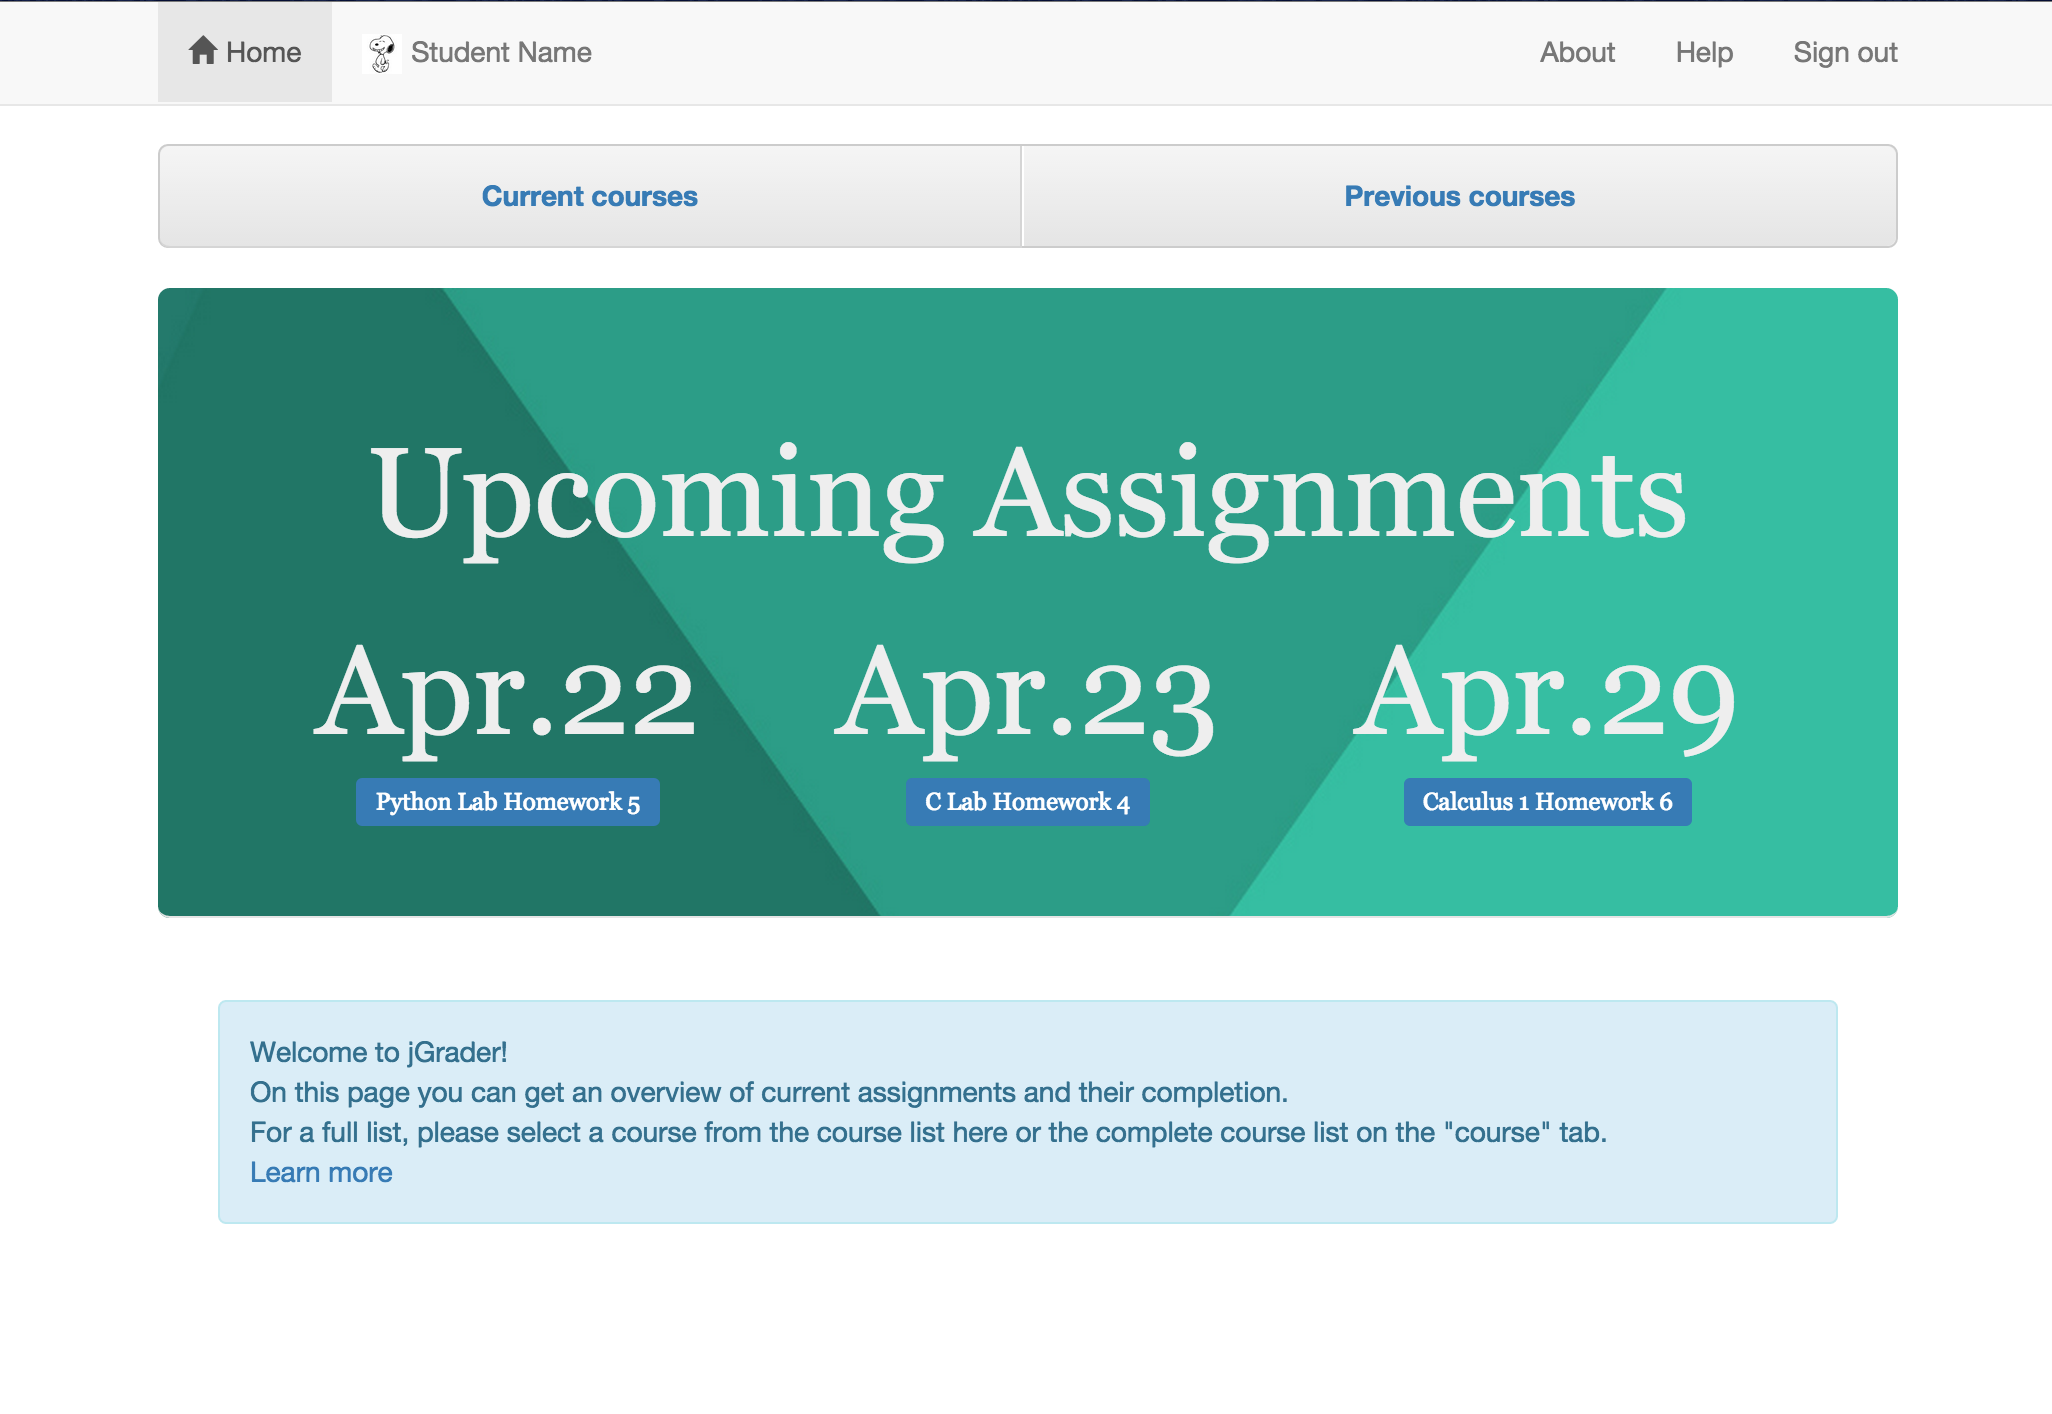
\includegraphics[width=\textwidth]{screenshots/StudentUpcomingAssignments.png}

\begin{itemize}

\item Students are provided with an overview of upcoming deadlines and how much of the tasks are done (e.g. if the student finished 4 out of 5 tasks it will visually show 80\%). This will help students remember all their deadlines.

\item Links on the visual representation of the percentages will allow students to quickly navigate to the assignments that are due.

\item To limit the information that is on the screen previous courses are only shown when the student clicks on the rider for previous courses. This ensures that the page provides an easily processable overview without clutter.

\item In the Enrolled Courses section, the student can access all courses he is currently enrolled in.

\end{itemize}
\newpage
\subsection{TA Landing Page (Nick)}
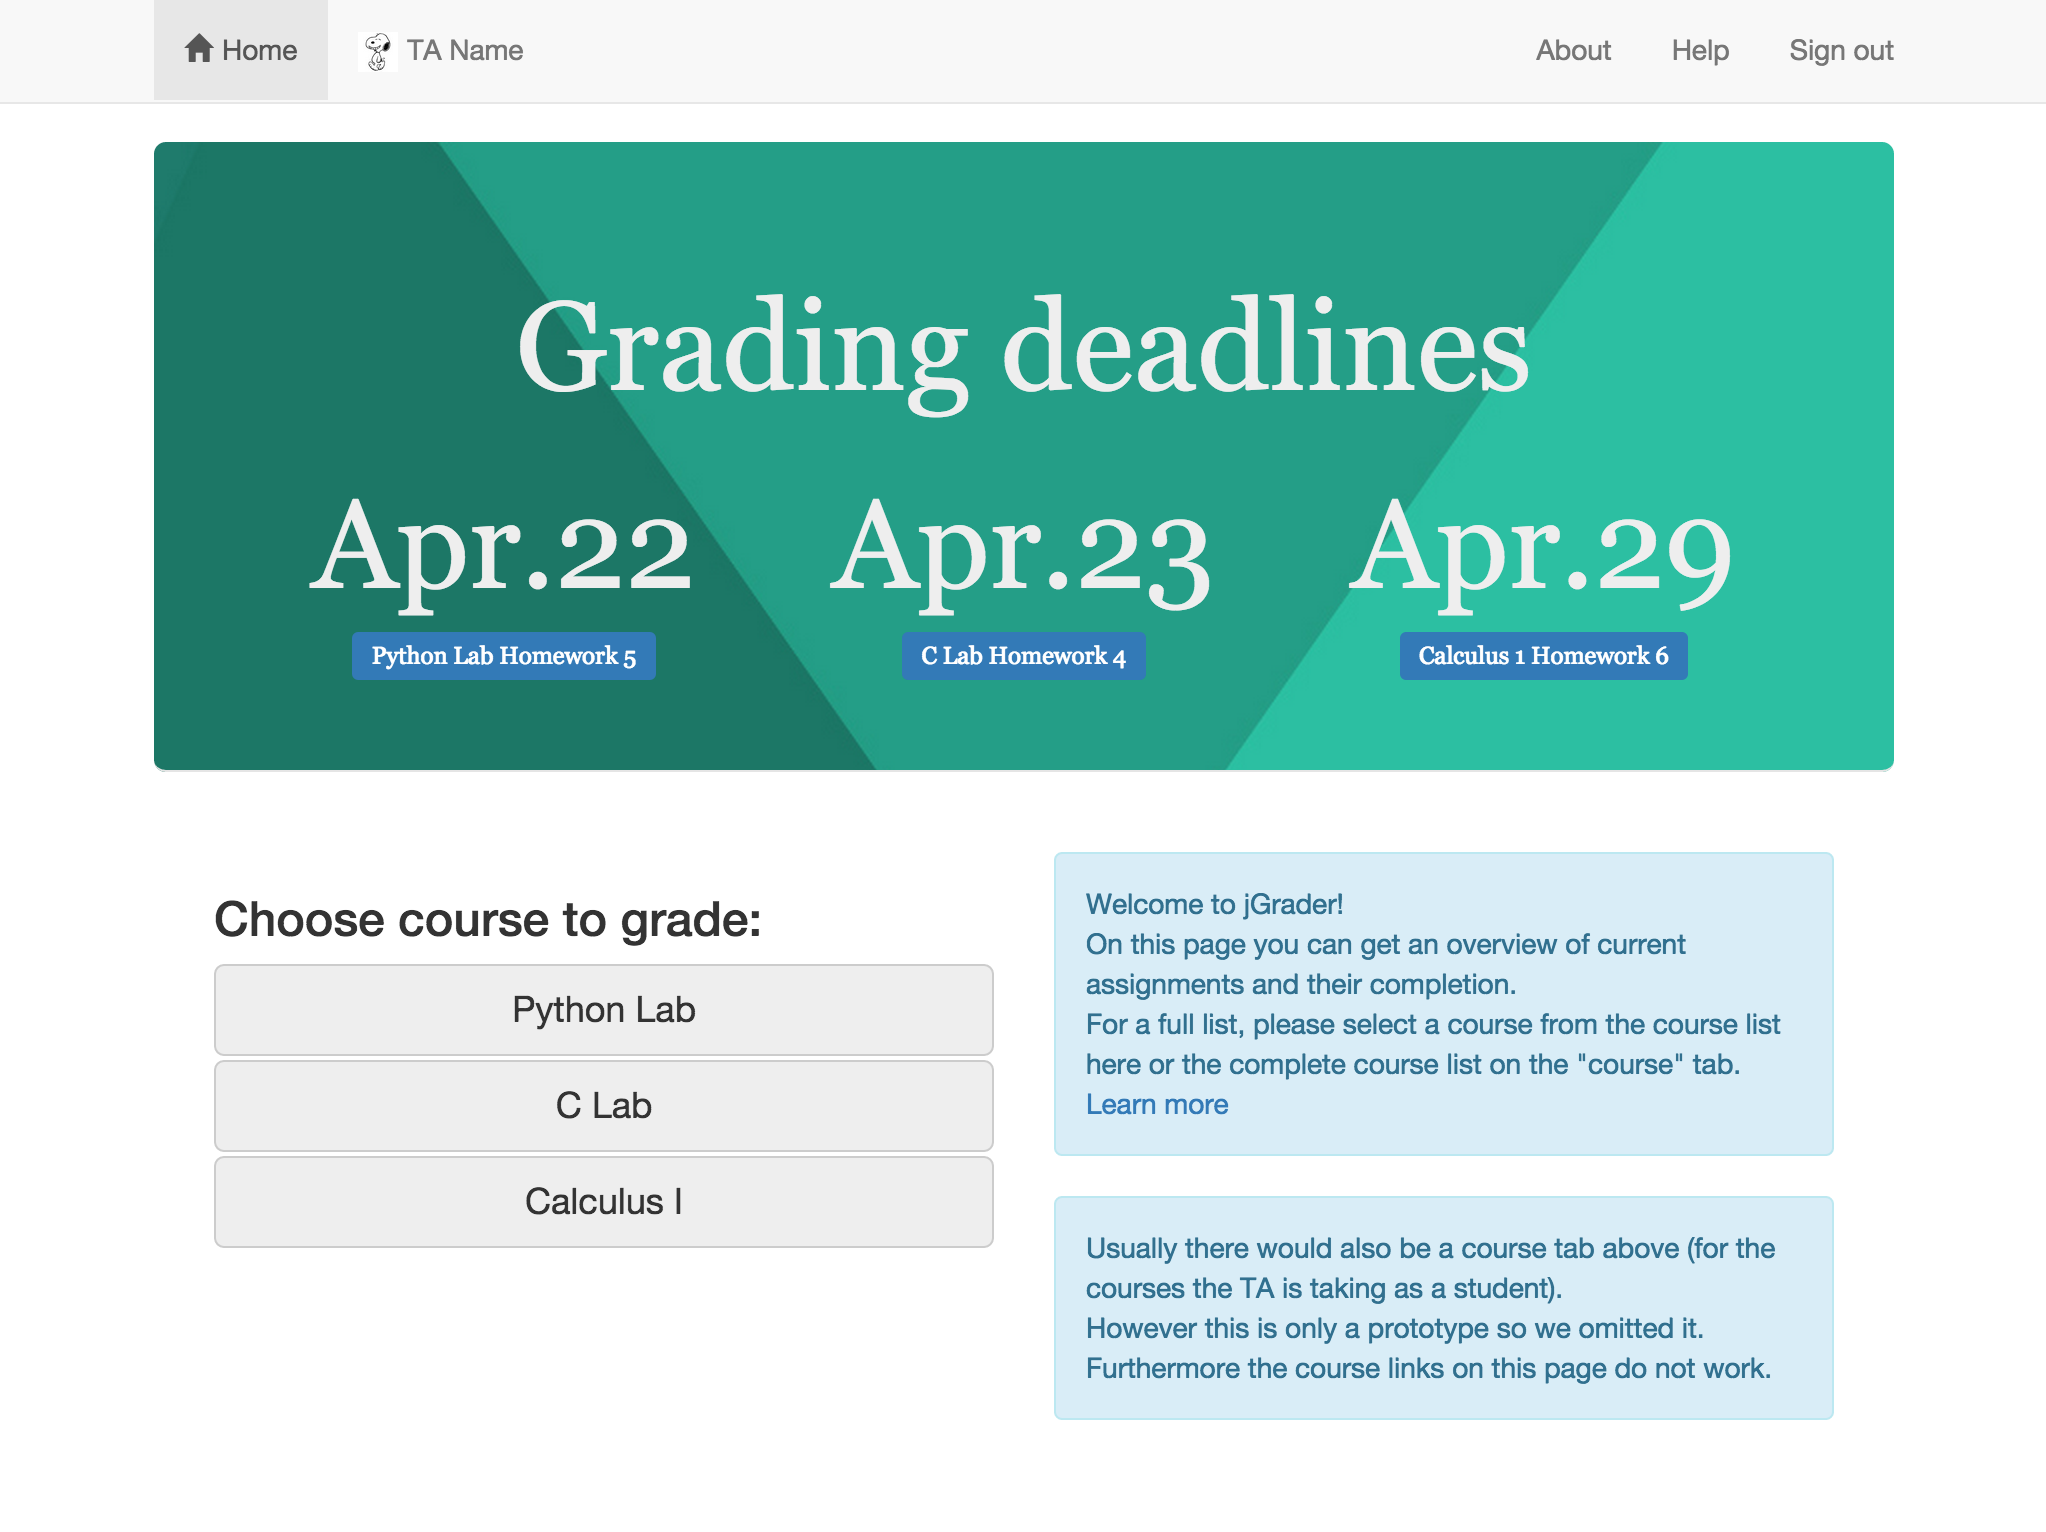
\includegraphics[width=\textwidth]{screenshots/TALandingPage.png}
The TA landing page is mostly the same as the student menu, and contains no major differentiation in the prototype beyond easy links to the grading pages for current courses. In a production environment, the current and previous courses would show any courses for which they have TA permissions. 

When the TA enters the grading overview page, they see a list of assignments for that course, along with the current status of the grading for the assignment. Colour coding helps the user to quickly navigate an information-dense page. Aqua indicates that grading is complete and there is no further action required. Yellow indicates that grading is partly finished, and orange indicates that grading has not started. Grey is used to indicate a non-actionable assignment that has received no submissions yet.\newpage

\subsection{Profile Pages (Tom)}
\ednote{Write this section}
\newpage

\subsection{Current courses page (Roxana)}

\includegraphics[width=.75\textwidth]{screenshots/CurrentCourses.png}

The previous courses page is very similar in design to the current courses page, with addition of simple marks to indicate whether the student passed or failed the completed course, and a tab bar to navigate through previous semesters.

Orienting the list of semesters horizontally versus the vertical orientation of the courses helps reinforce that the user is navigating through a different set of information than when they simply scroll through courses.

The semester list grows horizontally because it can be compacted better than the list of courses, is less likely to be used, and because it is more difficult to scroll horizontally than vertically on most computers. A less-used feature should use the more difficult action, leaving more natural actions for commonly used features.\newpage
\subsection{Previous courses page (Vlad)}

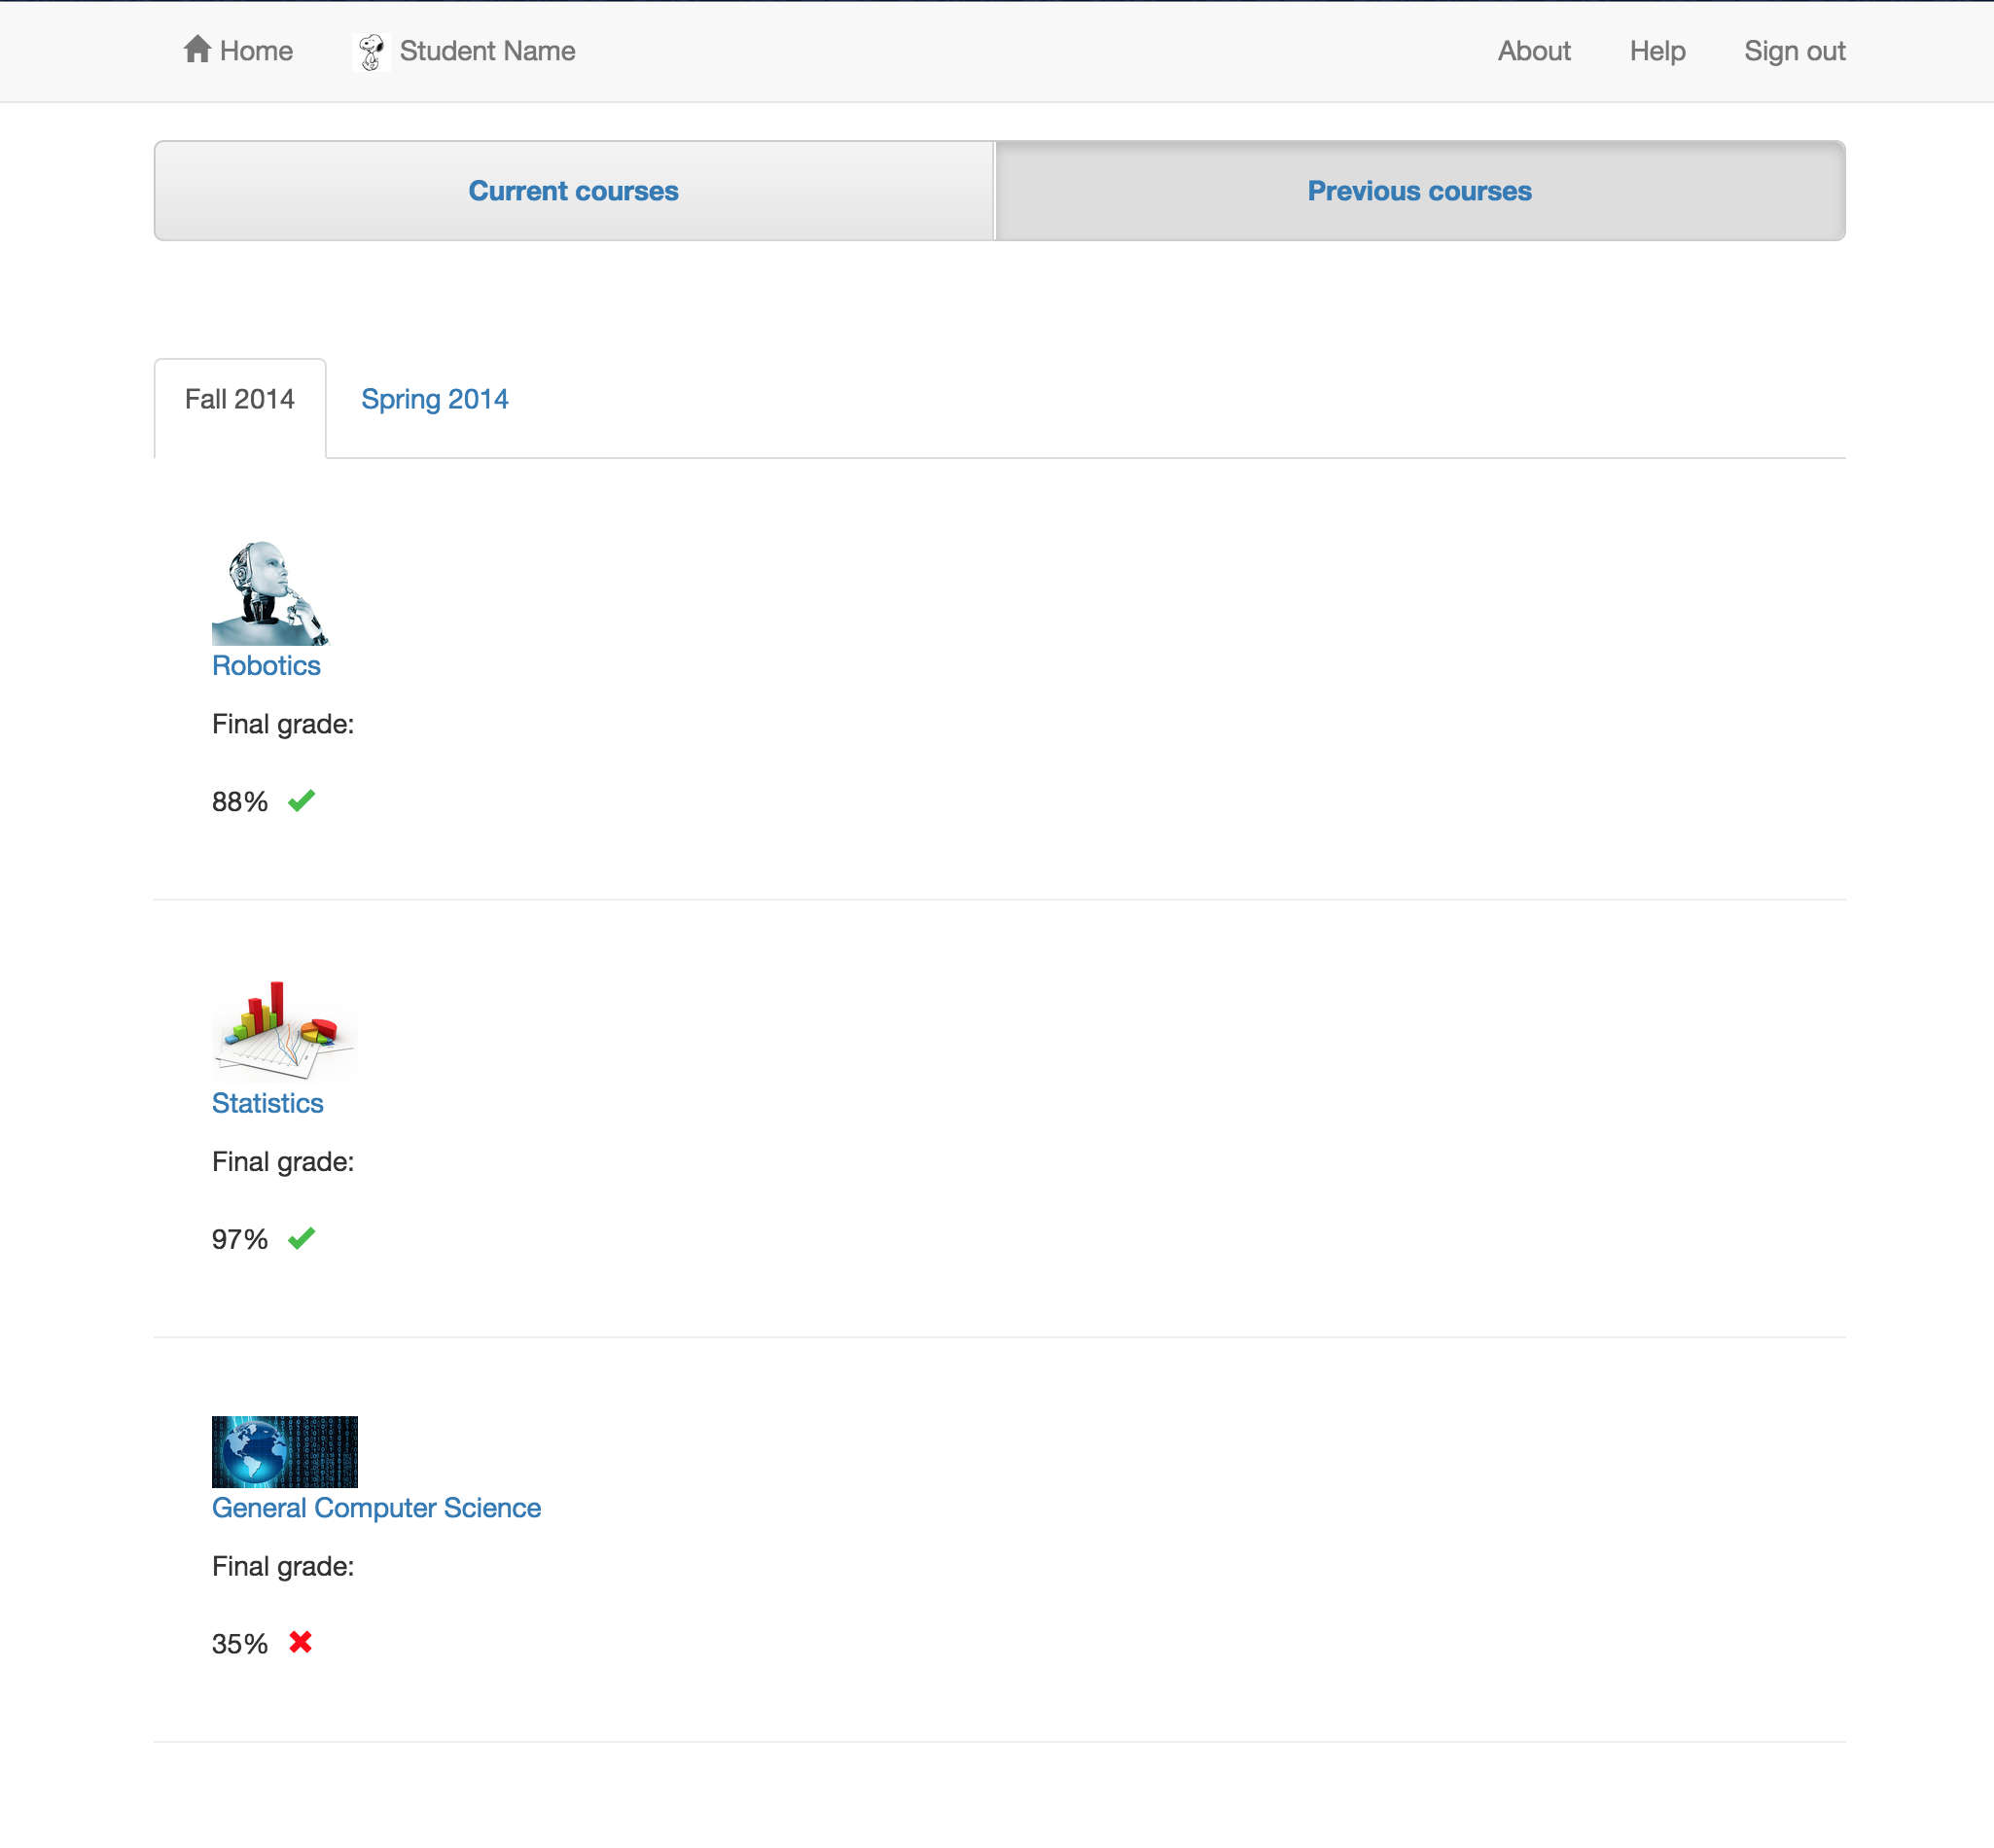
\includegraphics[width=\textwidth]{screenshots/PreviousCourses.png}

The current courses page features a sparse, left-justified layout in order to simplify the task of getting to the course page the user needs--minimal information beyond a grade overview, large \& attention-catching course icons, and the page navigation buttons is included. Following the rule-of-thirds by left-justifying the content helps the user process the information quicker.
\newpage

\subsection{Current Course Page}

Alice is taking Python this year which she uses our grading platform for. When she is is on the student landing page.\\
\includegraphics{../../screenshots/StudentLandingPage.png}\\
From there she realizes that the next assignment due is for Python Lab. Alice clicks on the \textit{Current courses} to have an overview of all her courses.\\
\includegraphics{../../screenshots/CurrentCourses}\\
Since she still has to do her Python homework assignment she navigates to the Python Lab.\\
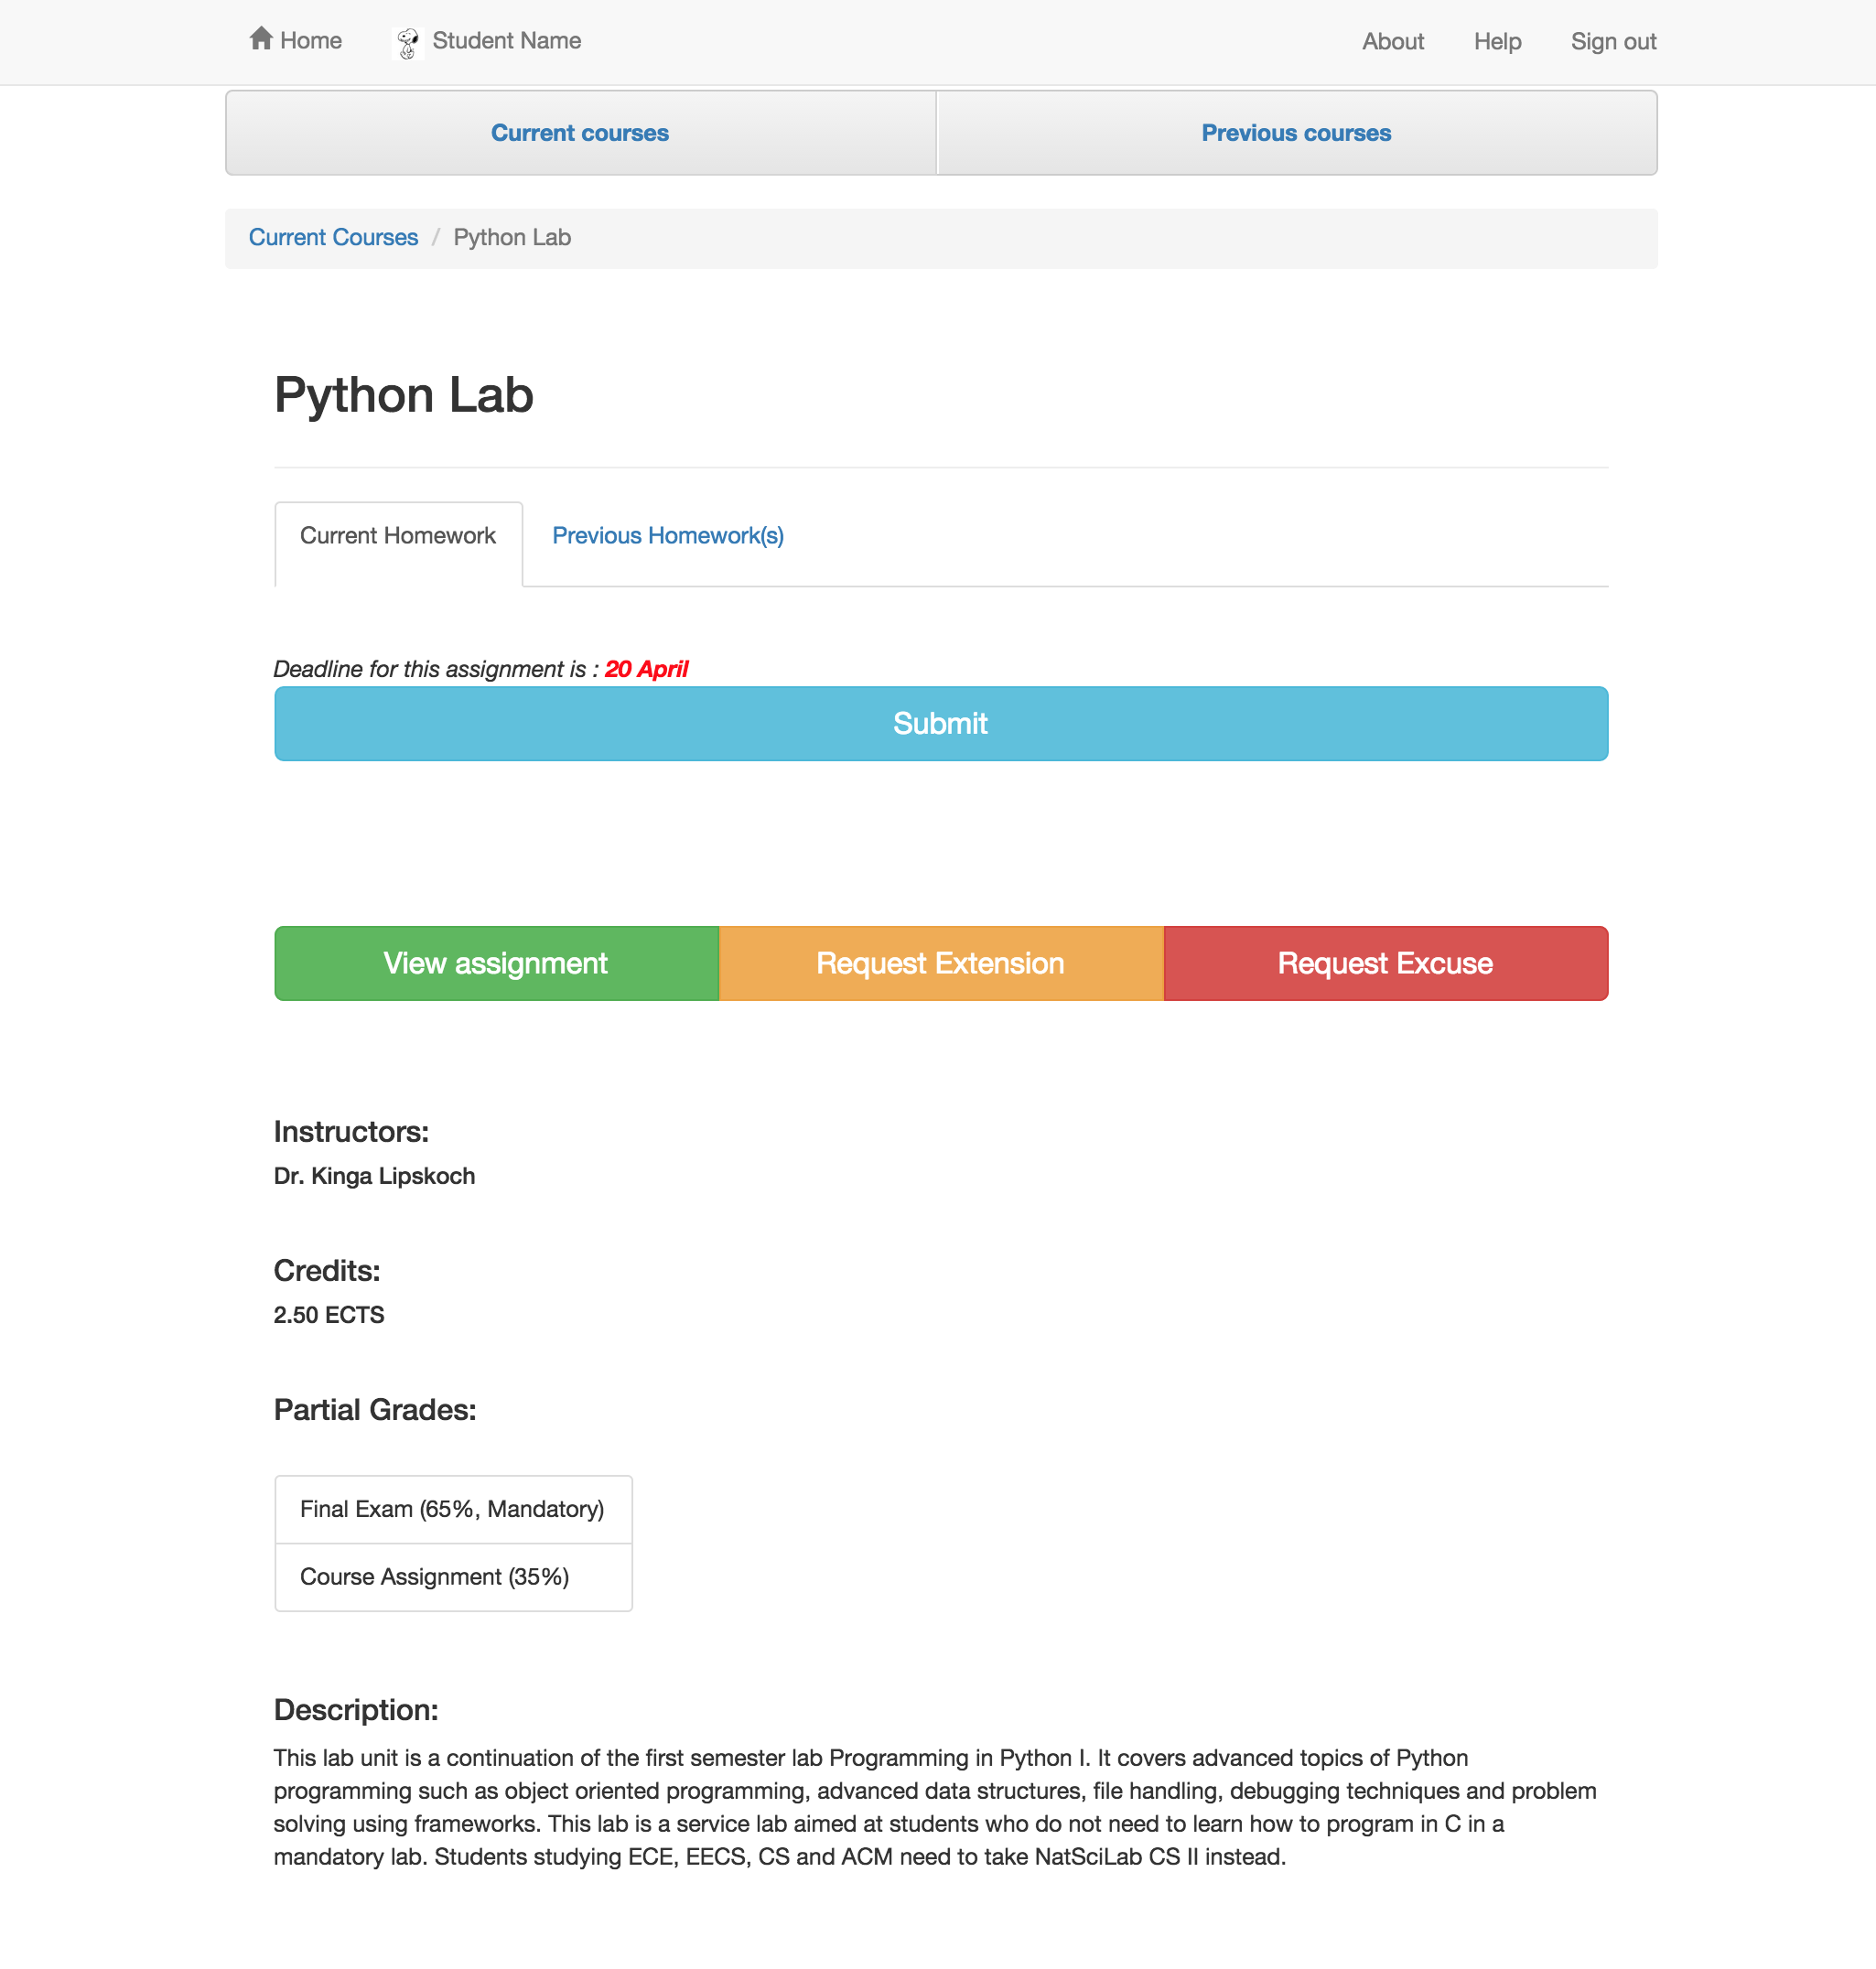
\includegraphics{../../screenshots/PythonLab}\\
The course page layout is designed to provide an easy to use and comprehensive dashboard for each course. It contains current assignments, previous assignments, tools to view further information, request extensions \& excuses, and an overview of the course grading breakdown, instructors, credits, and other important information.\\

On the top of the page Alice can choose the current homework screen or the previous homework Assignments screen. On the current homework screen the most frequently accessed elements are at the top of the screen to minimize scrolling and allow for easy accessibility. Hence the first information is when the deadline for the current assignment it and right below it is a huge submit button that cannot be missed. Apart from this it also has buttons to view the current assignment, to request and extension, and to request an excuse. The colors for the buttons are green, yellow, and red respectively which underlines how crucial the respective action is. E.g. requesting an excuse is a more crucial action than requesting an extension.\\

Below the buttons that allow Alice to perform actions, the course page offers information about the course and the grading criteria. Being naturally curious about the grades she received on previous homework assignments, she goes to that section and can see her previous submissions and the grades she received for them in a nicely formatted table.\\
\includegraphics{../../screenshots/PreviousHW}\\
Going back to the current homework page, Alice wants to now submit her current homework assignment. For that she clicks on the submit button and is redirected to the submission page.\\
\includegraphics[width=\textwidth]{../../screenshots/Exercise5}\\
This is easily designed so that Alice can drag and drop files in or simply select the file by clicking on it.\\

\newpage

\subsection{TA Grading Page (Nick)}

\begin{itemize}
\item Assignments, sorted in descending order by `'\% ungraded'`', followed by `'most distant due date in the past'`' are selected from a main TA dashboard for the course showing numbers of graded tasks, a list of students, and other information.

\item `'We placed the comment box before the grade box in order to encourage TAs to provide comments for grades; when tabbing through the page, the comment field will be selected first'`

\item Ample space is provided between assignment entries in order to reduce the chance of visual confusion. In a complete implementation, JavaScript would also be used to turn the currently selected row/row fields are in grey in order to further differentiate what's being edited.

\item A single submit grades button, which floats throughout the page for easy access, reduces the number of steps necessary to enter a grade, which is important for TAs when grading large numbers of small assignments.

\item Different sizes between the comment and grade fields provide further visual differentiation.
\end{itemize}
\newpage

%%%%%%%%%%%%%%%%%%%%%%%%%%%%%%%%%%%%%%%%%%%%%%%%%%%%%%%%%%%%%%%%%%%%%%%%%%%

\end{document}
